\chapter{Figures}

% ==========================================================================================
% Exploratory Data Analysis
% ==========================================================================================
\begin{figure}[H]
    \centering
    \fbox{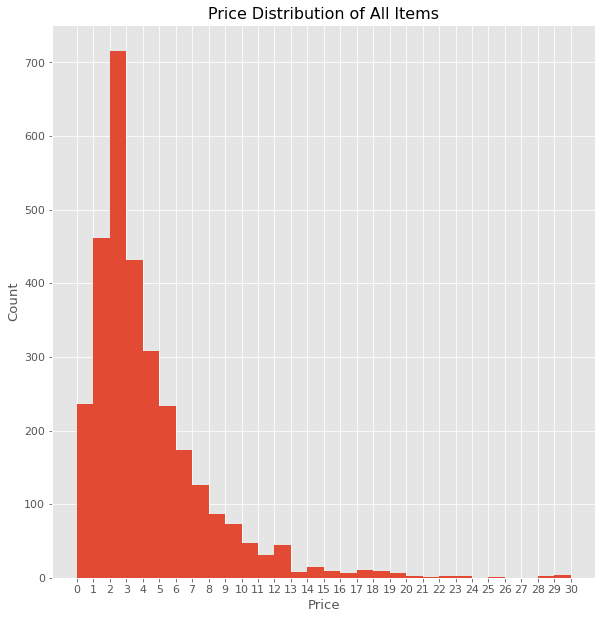
\includegraphics[width=0.9\textwidth]{figures/exploratory_data_analysis/price_all.png}}
    \caption{The distribution of the prices of all products.}
    \label{fig:price_all}
\end{figure}

\begin{figure}
    \centering
    \fbox{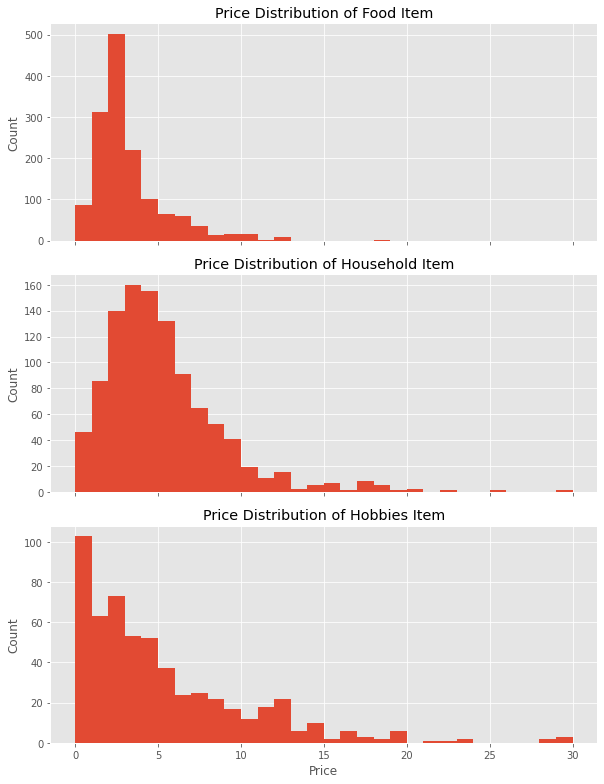
\includegraphics[width=0.98\textwidth]{figures/exploratory_data_analysis/price_dist_cats.png}}
    \caption{The price distribution of products in each product category.}
    \label{fig:price_cats}
\end{figure}

\begin{figure}
    \centering
    \fbox{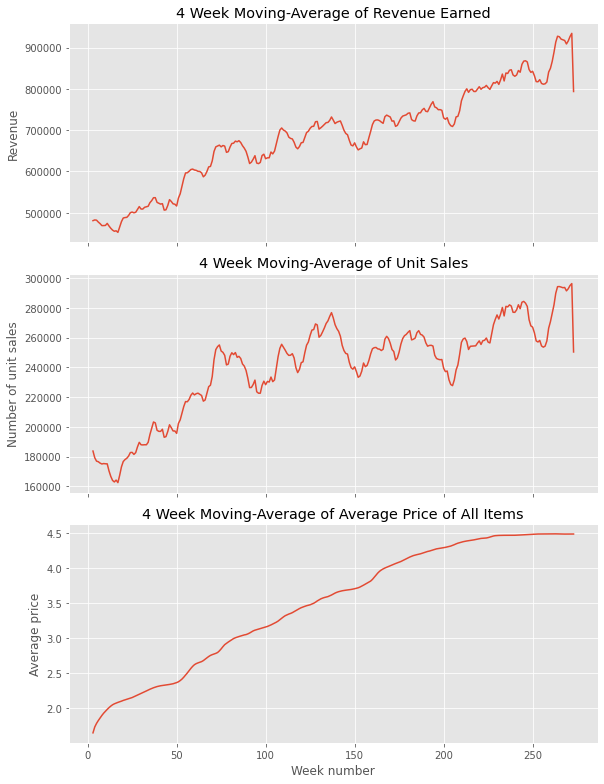
\includegraphics[width=0.98\textwidth]{figures/exploratory_data_analysis/4-week-ma.png}}
    \caption{4 week moving-average of revenue, unit sales, and average price of items.}
    \label{fig:ma_4week}
\end{figure}

% ==========================================================================================
% RESULTS
% ==========================================================================================

\begin{figure}
    \centering
    \fbox{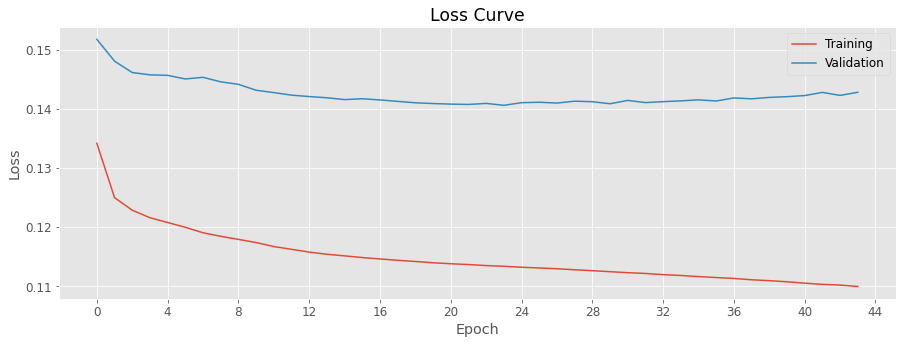
\includegraphics[width=0.95\textwidth]{figures/results/lstm_curve.png}}
    \caption{The learning curve of the LSTM model.}
    \label{fig:lstm_curve}
\end{figure}

\begin{figure}
    \centering
    \fbox{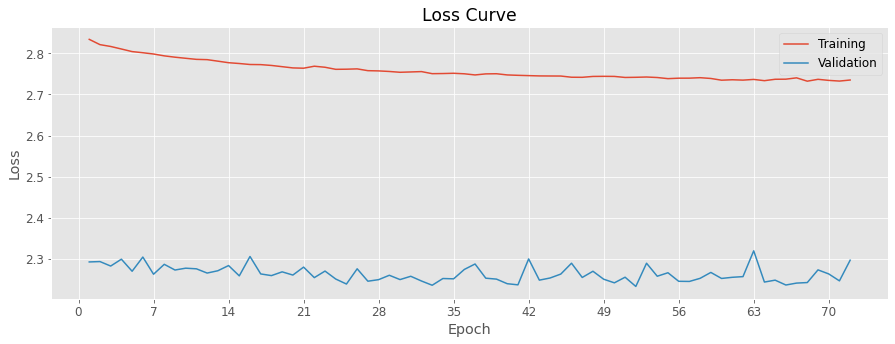
\includegraphics[width=0.95\textwidth]{figures/results/ann_curve.png}}
    \caption{The learning curve of the MLP model.}
    \label{fig:ann_curve}
\end{figure}

\begin{figure}
    \centering
    \fbox{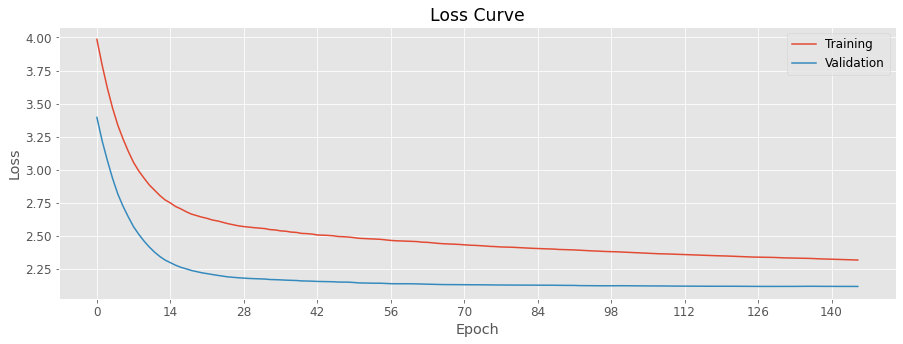
\includegraphics[width=0.95\textwidth]{figures/results/lgbm_curve.png}}
    \caption{The learning curve of the LGBM model.}
    \label{fig:lgbm_curve}
\end{figure}

\clearpage
\begin{figure}
\centering
    \subfloat[1-day ahead predictions on the training, validation, and test sets.]{
    	\label{subfig:lstm_sample1}
    	\fbox{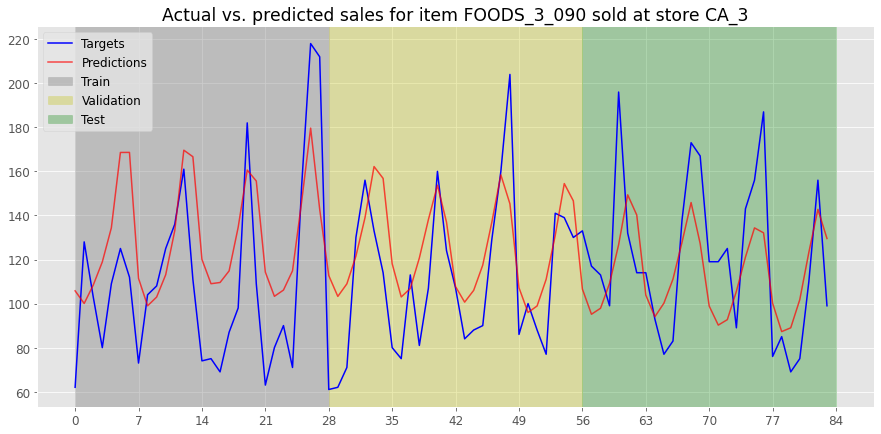
\includegraphics[width=0.95\textwidth]{figures/results/lstm_sample_preds.png}}
    	} 
    \vspace{5mm}
    \subfloat[28-days ahead predictions on the test set]{
    	\label{subfig:lstm_sample28}
    	\fbox{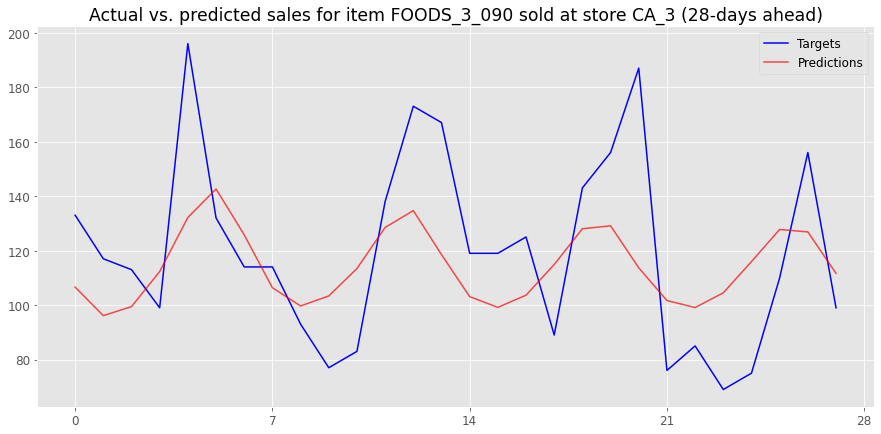
\includegraphics[width=0.95\textwidth]{figures/results/lstm_tst28_preds.png}}
    	}
    \vspace{2mm}
    \caption{Samples of LSTM predictions vs. the actual values.}
    \label{fig:lstm_samples}
\end{figure}

\begin{figure}
    \centering
    \fbox{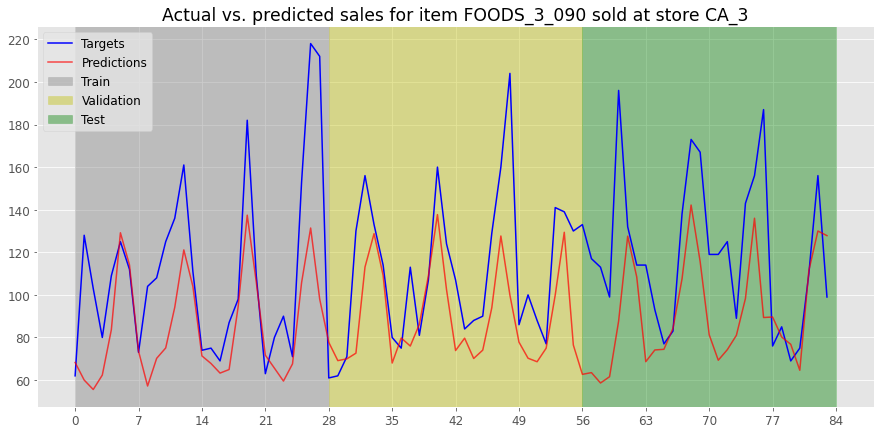
\includegraphics[width=0.95\textwidth]{figures/results/ann_sample_preds.png}}
    \caption{Samples of MLP predictions vs. the actual values.}
    \label{fig:ann_samples}
\end{figure}

\begin{figure}
    \centering
    \fbox{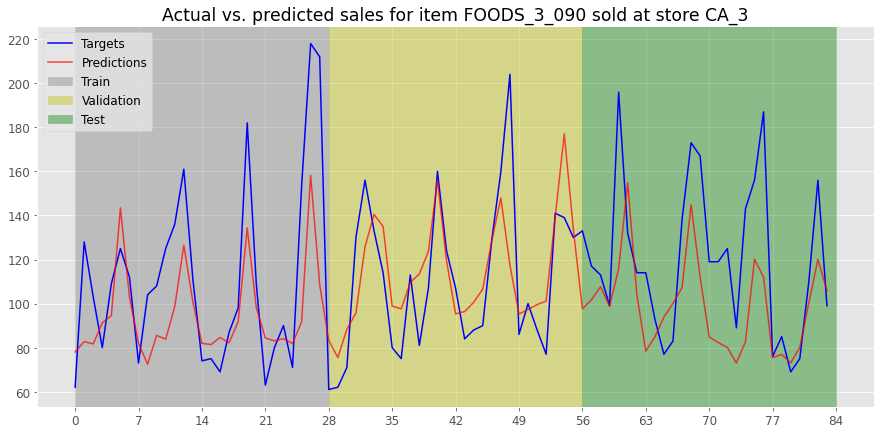
\includegraphics[width=0.95\textwidth]{figures/results/lgbm_sample_preds.png}}
    \caption{Samples of LGBM predictions vs. the actual values.}
    \label{fig:lgbm_samples}
\end{figure}

\begin{figure}
\centering
    \subfloat[1-day ahead predictions on the training, validation, and test sets.]{
    	\label{subfig:hyb_sample1}
    	\fbox{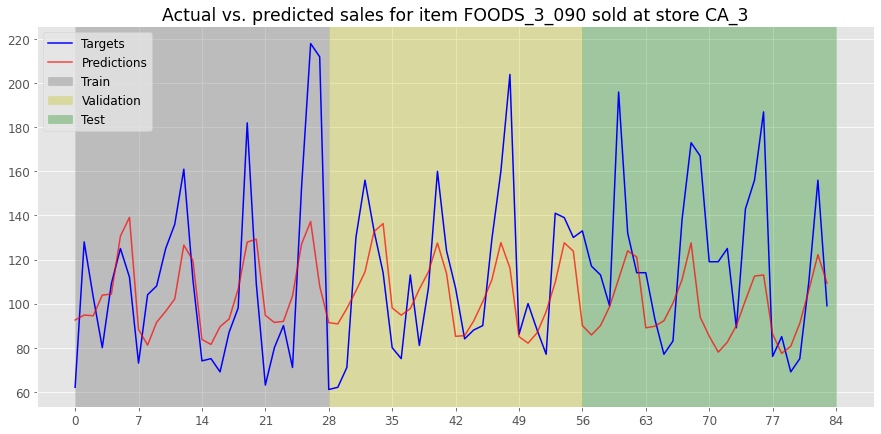
\includegraphics[width=0.95\textwidth]{figures/results/hyb_sample_preds.png}}
    	} 
    \vspace{5mm}
    \subfloat[28-days ahead predictions on the test set]{
    	\label{subfig:hyb_sample28}
    	\fbox{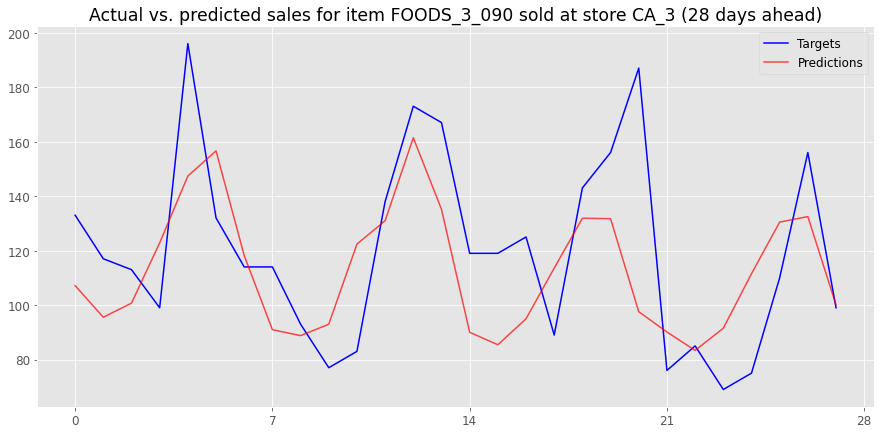
\includegraphics[width=0.95\textwidth]{figures/results/hyb_tst28_preds.png}}
    	} 
    \vspace{2mm}
    \caption{Samples of the LSTM-LGBM hybrid model's predictions vs. the actual values.}
    \label{fig:hyb_samples}
\end{figure}

\clearpage
\begin{figure}
    \centering
    \fbox{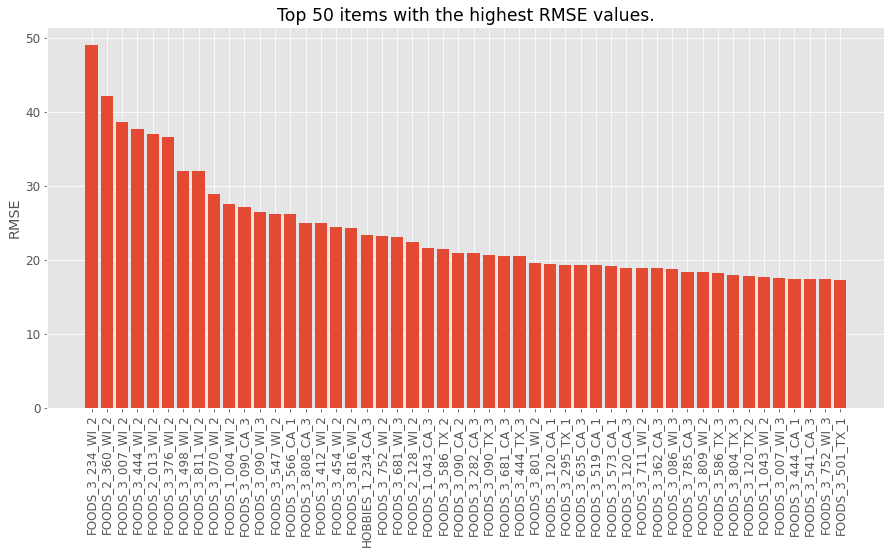
\includegraphics[width=0.95\textwidth]{figures/results/lstm_worst.png}}
    \caption{Top 50 items with the highest RMSE for the LSTM model.}
    \label{fig:lstm_worst}
\end{figure}

\begin{figure}
    \centering
    \fbox{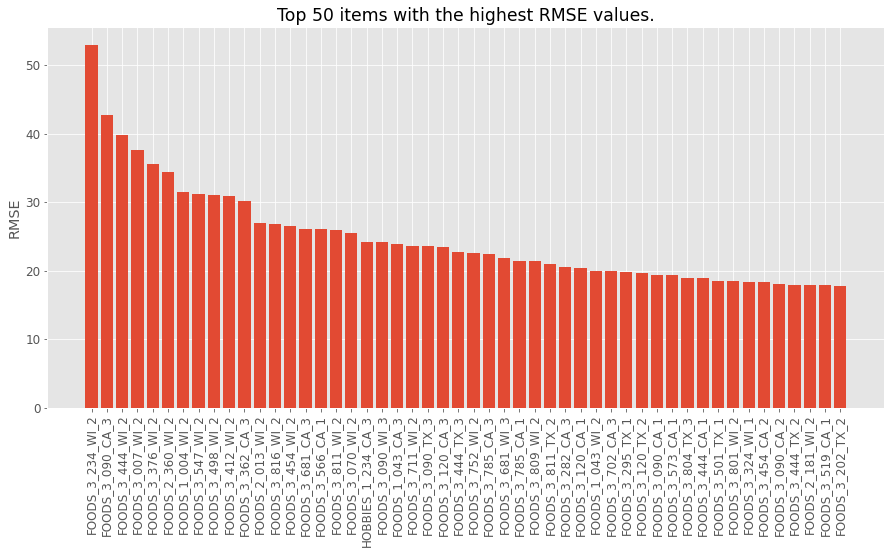
\includegraphics[width=0.95\textwidth]{figures/results/ann_worst.png}}
    \caption{Top 50 items with the highest RMSE for the MLP model.}
    \label{fig:ann_worst}
\end{figure}

\begin{figure}
    \centering
    \fbox{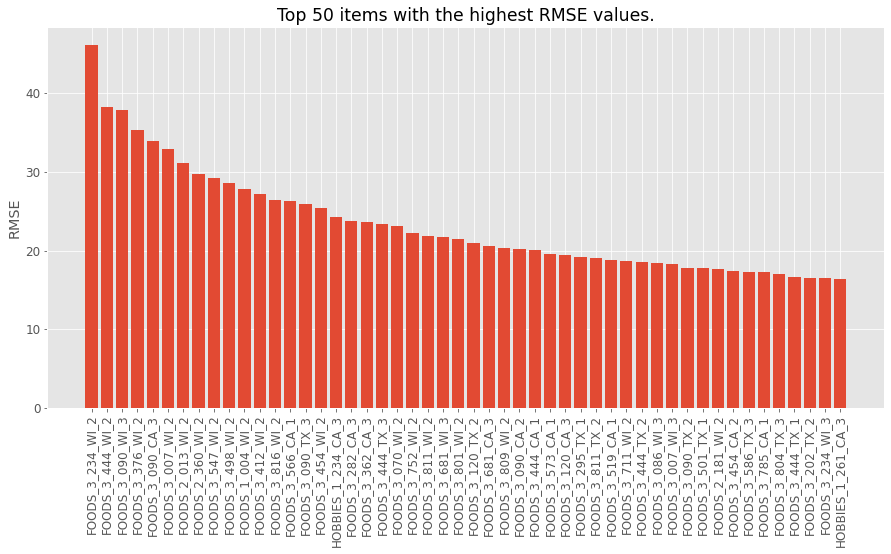
\includegraphics[width=0.95\textwidth]{figures/results/lgbm_worst.png}}
    \caption{Top 50 items with the highest RMSE for the LGBM model.}
    \label{fig:lgbm_worst}
\end{figure}

\begin{figure}
    \centering
    \fbox{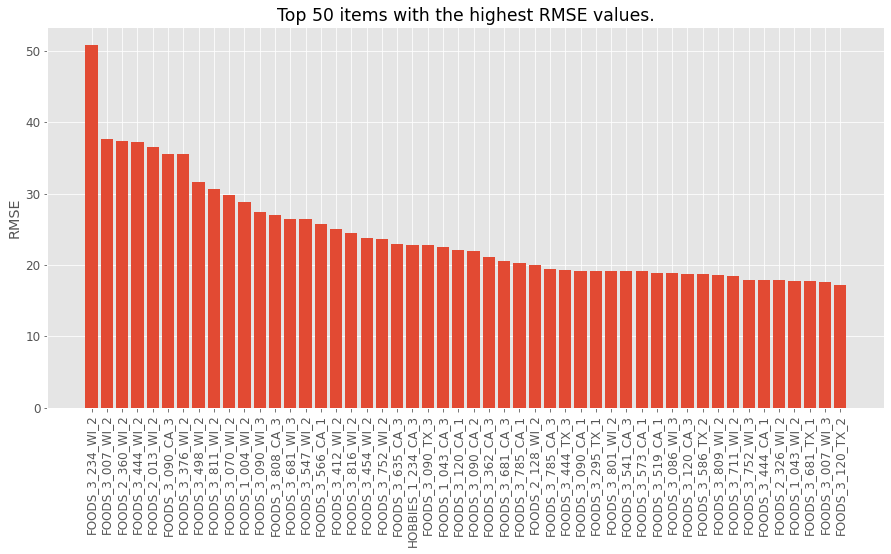
\includegraphics[width=0.95\textwidth]{figures/results/hyb_worst.png}}
    \caption{Top 50 items with the highest RMSE for the LSTM-LGBM hybrid model.}
    \label{fig:hyb_worst}
\end{figure}